\subsubsection{Overview of The Performances}
~
\begin{figure}[bth]
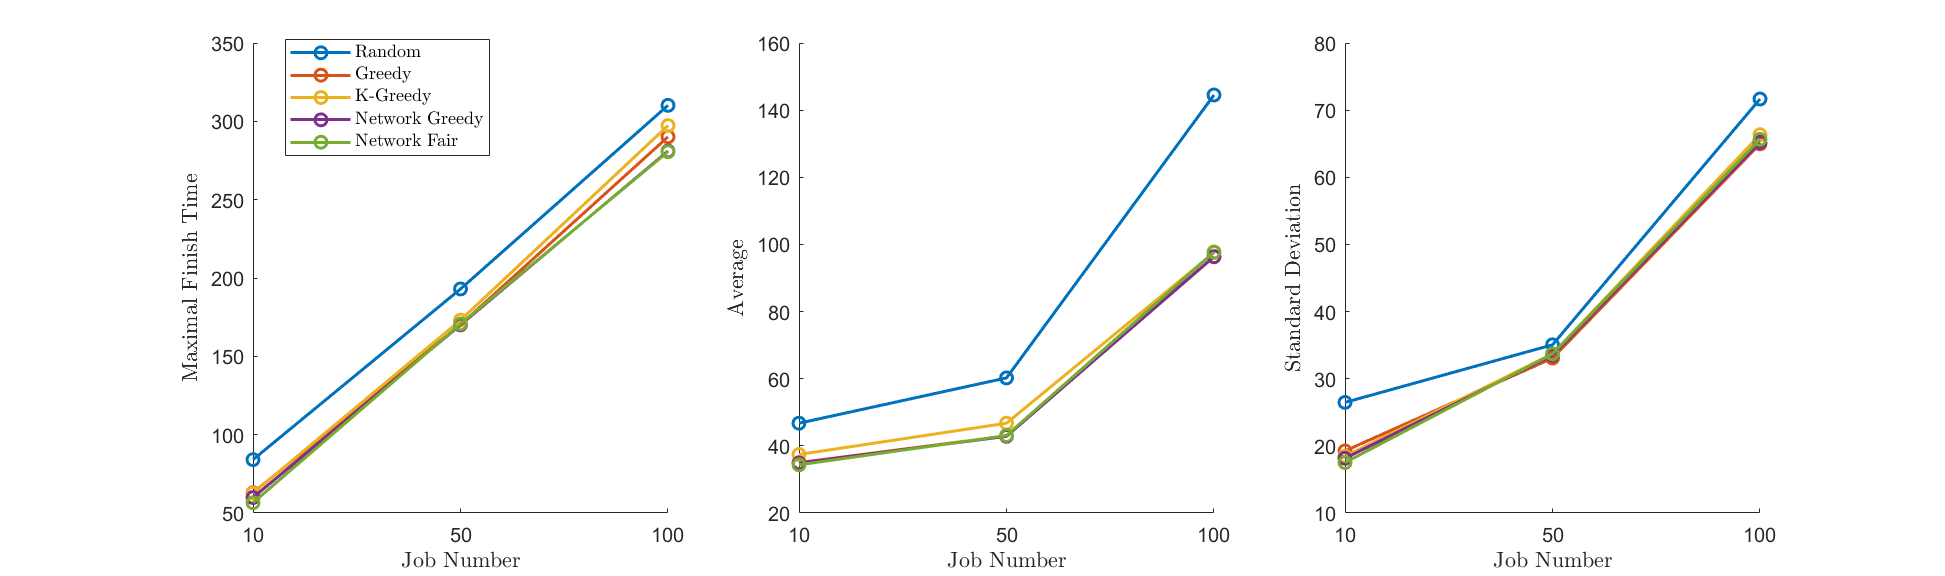
\includegraphics[width=1\textwidth]{figure/60.png}
\centering
\caption{60\% small jobs} \label{fig-60}
\end{figure}

\begin{figure}[bth]
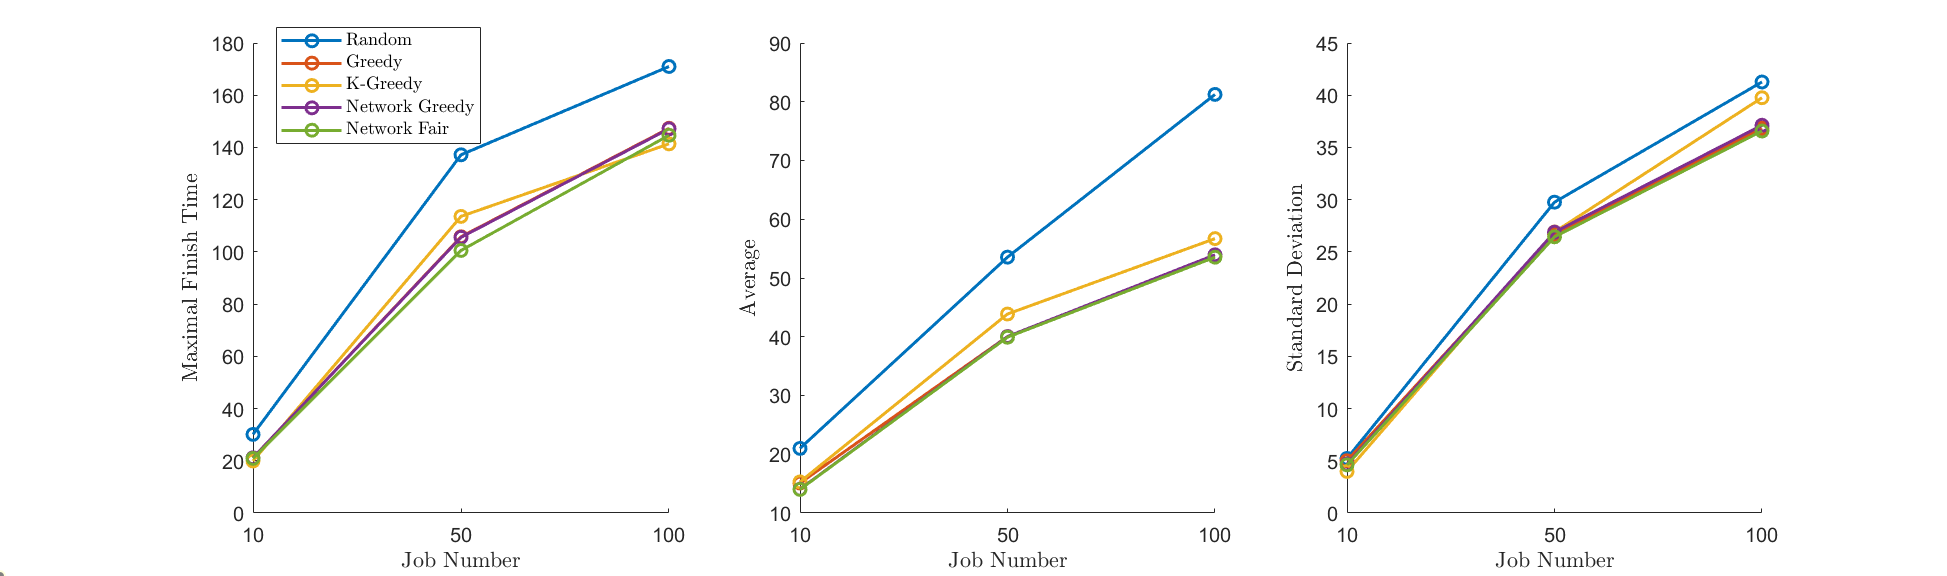
\includegraphics[width=1\textwidth]{figure/80.png}
\centering
\caption{80\% small jobs} \label{fig-80}
\end{figure}

We generate data with different job number and different proportion of small jobs. Fig. \ref{fig-60} and Fig. \ref{fig-80} show the maximal finish time, average finish time and its standard deviation.
We can observe the following outcome 
\begin{enumerate}
    \item Greedy and Fair Approach are much better than the random baseline. 
    \item K-Greedy Approach is not that stable but can sometimes yields a better solution.
    \item Greedy Approach and Network-Based Greedy have similar outcome.
    \item Network-Based Fair Approach have a high probability to achieve a best solutions in all metrics, with job amount and small job proportion are large.
\end{enumerate}